\documentclass{beamer}[fontset=windows]
\usepackage{ctex, hyperref}
\usepackage[T1]{fontenc}
\usepackage[backend=bibtex,bibstyle=gb7714-2015,citestyle=gb7714-2015]{biblatex}
\setlength{\bibitemsep}{3bp}
\addbibresource{ref.bib}
\renewcommand*{\bibfont}{\zihao{5}\linespread{1.27}\selectfont}
\usefonttheme[onlymath]{serif}
% other packages
\usepackage{latexsym,amsmath,xcolor,multicol,booktabs,calligra}
\usepackage{graphicx,pstricks,listings,stackengine}

\author{吴熙楠}
\title{钙钛矿发光材料}
\institute{北京大学物理学院}
\date{\today}
\usepackage{PKU}
% defs
\def\cmd#1{\texttt{\color{red}\footnotesize $\backslash$#1}}
\def\env#1{\texttt{\color{blue}\footnotesize #1}}
\definecolor{deepblue}{rgb}{0,0,0.5}
\definecolor{deepred}{rgb}{0.6,0,0}
\definecolor{deepgreen}{rgb}{0,0.5,0}
\definecolor{halfgray}{gray}{0.55}

\lstset{
	basicstyle=\ttfamily\small,
	keywordstyle=\bfseries\color{deepblue},
	emphstyle=\ttfamily\color{deepred},    % Custom highlighting style
	stringstyle=\color{deepgreen},
	numbers=left,
	numberstyle=\small\color{halfgray},
	rulesepcolor=\color{red!20!green!20!blue!20},
	frame=shadowbox,
}


\begin{document}
	
	\kaishu
	\begin{frame}
		\titlepage
    \begin{figure}[htpb]
    	\begin{center}
    		
\includegraphics[width=0.2\linewidth]{pic/PKU_logo.png}
    	\end{center}
    \end{figure}
	\end{frame}
	
	\begin{frame}
		\tableofcontents[sectionstyle=show,subsectionstyle=show/shaded/hide,subsubsectionstyle=show/shaded/hide]
	\end{frame}
\section{金属卤化物钙钛矿及其性质}
\subsection{金属卤化物钙钛矿的基本概念}
\begin{frame}
	\begin{itemize}\small{
		\item 1839年德国矿物学家 Gustav Rose 发现了$ CaTiO_{3}$矿石,并以俄国矿物学家 LevPerovski的名字命名(Perovskite)。
		\item 金属卤化物钙钛矿结构通式也符合$ABX_{3}$\footnote{定义容错因子$t=\frac{R_{A}+R_{X}}{\sqrt{2}(R_{B}+R_{X})}$,典型的钙钛矿结构$0.78\le t\le 1.05$},但A位离子主要是甲铵($MA^{+}$)、甲脒($FA^{+}$)或者铯($Cs^{+}$)等一价阳离子,B 位离子主要 IV 主族的二价铅($Pb^{2+}$)或锡($Sn^{2+}$)离子,X位主要是负一价卤素离子,包括 $Cl^{-}$, $Br^{-}$和 $I^{-}$。}
	\end{itemize}
	\begin{figure}[H]
	\centering
	\hspace{2em}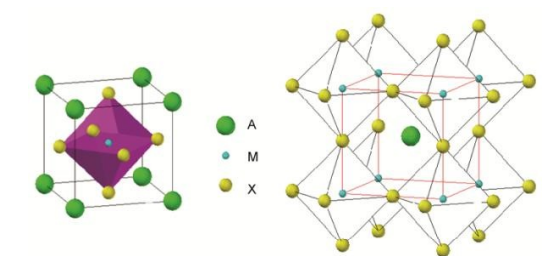
\includegraphics[width=.5\linewidth]{pic/1.png}
	\caption{金属卤化物钙钛矿结构示意图
	}
\end{figure}
\end{frame}
\subsection{金属卤化物钙钛矿的基本光学性质}
\begin{frame}
	\begin{itemize}
		\item 作为一种晶体半导体材料,金属卤化物钙钛矿的一大显著优势是发光可以在$400-800 nm$ 的范围内连续可调,覆盖了整个可见光区域\cite{stranks2015metal}。最常见的调节钙钛矿发光峰位的方法是改变钙钛矿元素种类,A, M, X 三种离子的选取对钙钛矿的能带结构都有一定影响,从而导致发光峰位的移动\cite{sutherland2016perovskite}。
		\item 如$ CsPbI_{3}$钙钛矿的禁带宽度是$1.73eV$\cite{swarnkar2016quantum},$CsPbBr_{3}$钙钛矿的禁带宽度是$2.35 eV$\cite{becker2018bright}, $CsPbCl_{3}$ 钙钛矿的禁带宽度则达到 $3.06 eV$\cite{becker2018bright}。通过选择合适卤素元素并适当混合(如 $CsPb(Cl/Br)_{3}$,$CsPb(Br/I)_{3}$等),就可以得到发光覆盖$400-700nm$的$CsPbX_{3}$ 钙钛矿。
	\end{itemize}
\end{frame}	
\begin{frame}
	\begin{figure}[H]
		\centering
		\hspace{2em}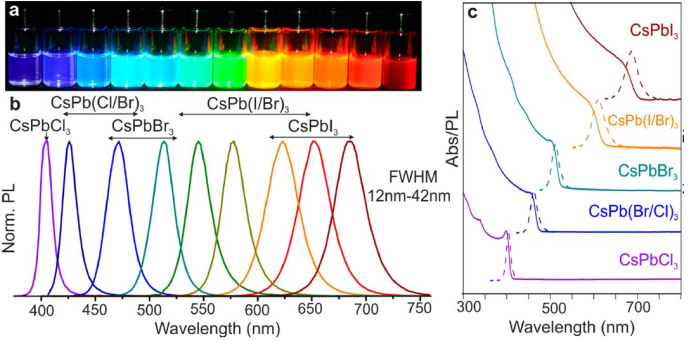
\includegraphics[width=.75\linewidth]{pic/2.png}
		\caption{$CsPbX_{3}$钙钛矿组分调控实现光谱调控\cite{yakunin2015low}
		}
	\itshape
	$a.$紫外灯$365 nm$下的 $CsPbX_{3}$ 钙钛矿溶液照片;$b.CsPbX_{3}$钙钛矿的荧光光谱;$c.$典型$ CsPbX_{3} $钙钛矿的吸收与荧光光谱
	\end{figure}
\end{frame}
\begin{frame}
	\begin{itemize}
		\item 金属卤化物钙钛矿的另一个重要的优点是窄发光峰宽带来的高色纯度。作为一种直接带隙半导体材料,钙钛矿的荧光来自于带边自由载流子的直接复合(如三维钙钛矿,激子束缚能较小,基本不受到晶体尺寸的影响)或带边激子直接复合(纳米结构钙钛矿,激子束缚能较大的情况),因此钙钛矿的荧光半峰宽非常窄。
	\end{itemize}
	\begin{figure}[H]
	\centering
	\hspace{2em}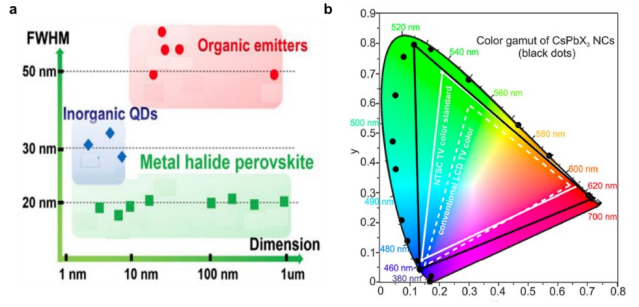
\includegraphics[width=.7\linewidth]{pic/3.png}
	\caption{$a.$钙钛矿、量子点、有机发光材料的半峰宽对比;$b.$钙钛矿发光材料色域覆盖范围\cite{yakunin2015low}
	}
\end{figure}
\end{frame}
\begin{frame}
	\begin{block}{荧光量子产率}
		\begin{itemize}
			\item 单位时间内,发光材料发射的光子数与吸收的光子数之比。
			\item 考虑到材料吸收光子产生的激发态(自由载流子和激子等)最终会通过各种辐射复合通道和非辐射复合通道复合。$PLQY=\dfrac{k_{r}}{k_{r}+k_{nr}}$
			\item 辐射复合:是自由载流子的双分子复合也可以是电子空穴对形成激子后的单分子复合;非辐射复合:各种缺陷和陷阱态造成的单分子复合,在激发密度很高的情况下,俄歇复合也会造成严重的非辐射复合。
			\item 钙钛矿量子点由于量子限域效应,激子束缚能较大,同时俄歇复合常数较小,因此在得到较好的表面钝化过后会量子产率非常高,接近$100\%$\cite{li2016cspbx3}(其余荧光LED材料在激发浓度较小时$PLQY$会明显下降)。
		\end{itemize}
	\end{block}
\end{frame}
\section{钙钛矿二极管}
\subsection{钙钛矿二极管基本构成}
\begin{frame}
	\begin{block}{$PeLED$结构}
		\begin{itemize}\small{
			\item 一个完整的 $PeLED$ 器件至少有以下五个功能层组成,依次包括阴极、电子传输层、钙钛矿发光层、空穴传输层和阳极。
			\item 阴极材料负责向电子传输层注电子,一般以低功函数的材料,如 $Ca, Al,Ag$ 等金属较为多见。
			\item 电子传输层将阴极注入的电子传输并注入到发光层,要求电子迁移率高,导带 位置合适,常见的有$ ZnO,TiO_{2} $等氧化物纳米晶或者部分小分子有机物材料。
			\item 发光层为钙钛矿,注入的电子和空穴在此复合,因此要求荧光量子产率尽量高,同时价带导带能级位置合适以满足载流子平衡注入的要求。
			\item 空穴传输层将阳极注入的空穴运输并注入到发光层,因此要求空穴迁移率高,价带位置合适,常见的有$ NiO$及部分有机物材料。
			\item 阳极负责向空穴传输层注入空穴,一般要求高功函数的材料,常见有铟锡氧化物透明导电薄膜($ITO$),氟掺杂的 $SnO_{2}$透明导电薄膜(FTO)和金属 $Au $等。}
		\end{itemize}
	\end{block}
\end{frame}
\begin{frame}
	\begin{figure}[H]
		\centering
		\hspace{2em}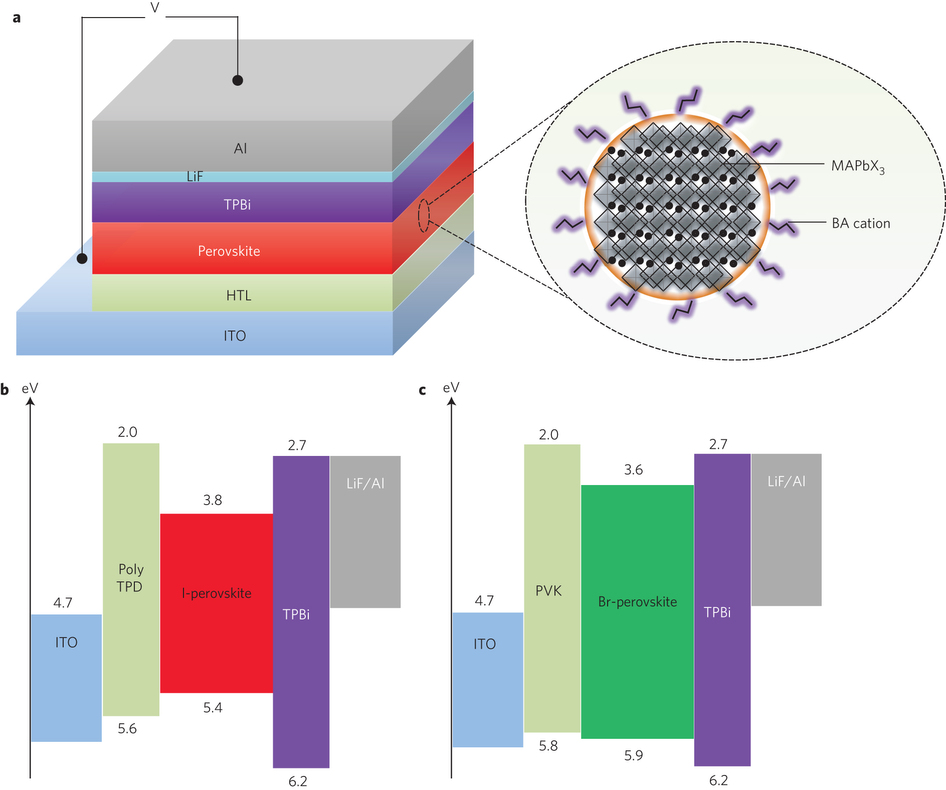
\includegraphics[width=.75\linewidth]{pic/6.jpg}
		\caption{钙钛矿发光二极管结构图及能量图
		}
	\end{figure}
\end{frame}
\begin{frame}
	\begin{block}{$PeLED$工作原理}
		\begin{itemize}\small{
			\item 注入的电子和空穴在发光层中相遇,形成激子后发生辐射复合或电子和空穴作为自由载流子直接发生双分子复合最后复合产生的光子穿过各个功能层后射出器件。
			\item 钙钛矿层的折射率一般比较大(如$FAPbI_{3}$ 折射率为 $2.7$),且通常钙钛矿材料发光是各向同性的,因此,考虑到全反射条件的限制,将有很大一部分辐射出来的光子无法射出器件。
			\item $PeLED$ 器件的总厚度往往不超过 $300 nm$,发光中心到金属电极的距离小于半波长。此时 $PeLED$ 中将出现明显的近场光学效应,金属电极会带来强烈的表面等离子共振吸收,造成大量光损耗。
			\item 钙钛矿消光系数很高($\sim 10^{4}cm^{-1}$),在部分钙钛矿比较厚的 $PeLED$ 器件中存在显著的自吸收现象,也可能会造成光子的消耗\cite{cho2020role}。 
			\item 目前在每层不增加任何光提取情况下能达到最大出光效率为$20\%\sim 30\%$
		}
		\end{itemize}
	\end{block}
\end{frame}
\subsection{钙钛矿二极管的特点}
\begin{frame}
	\begin{itemize}\small{
		\item  $PeLED$发光层的沉积过程伴随着钙钛矿的形成与结晶的过程,薄膜沉积工艺不但影响钙钛矿薄膜的形貌,也极大地影响着钙钛矿膜的发光性质($OLED$ 与 $QLED$ 都需要先合成发光材料,然后再蒸镀、旋涂、喷墨打印等方法沉积成发光层,沉积过程原则上只影响发光层的形貌而不会影响发光性质)。
		\item $PeLED$的离子迁移问题(钙钛矿器件稳定性差的罪魁祸首):由于钙钛矿本质上是一种离子晶体,当有外加电场存在时,钙钛矿中的离子(主要是卤素离子)会从晶体结构比较“脆弱”的地方,如晶界、表面等存
		在大量缺陷的地方开始发生移动,从而导致器件性能的衰减\cite{wang2016stability}(解决方法暂时只有表面处理钝化)。
		\item $PeLED$的迟滞现象:受到离子迁移的影响,$PeLED$ 的电流-亮度-电压曲线和效率-电压曲线在正扫和反扫是不重合的(解决方法暂时也只有表面处理钝化)。
	}
	\end{itemize}
\end{frame}
\begin{frame}
	\begin{figure}[H]
		\centering
		\hspace{2em}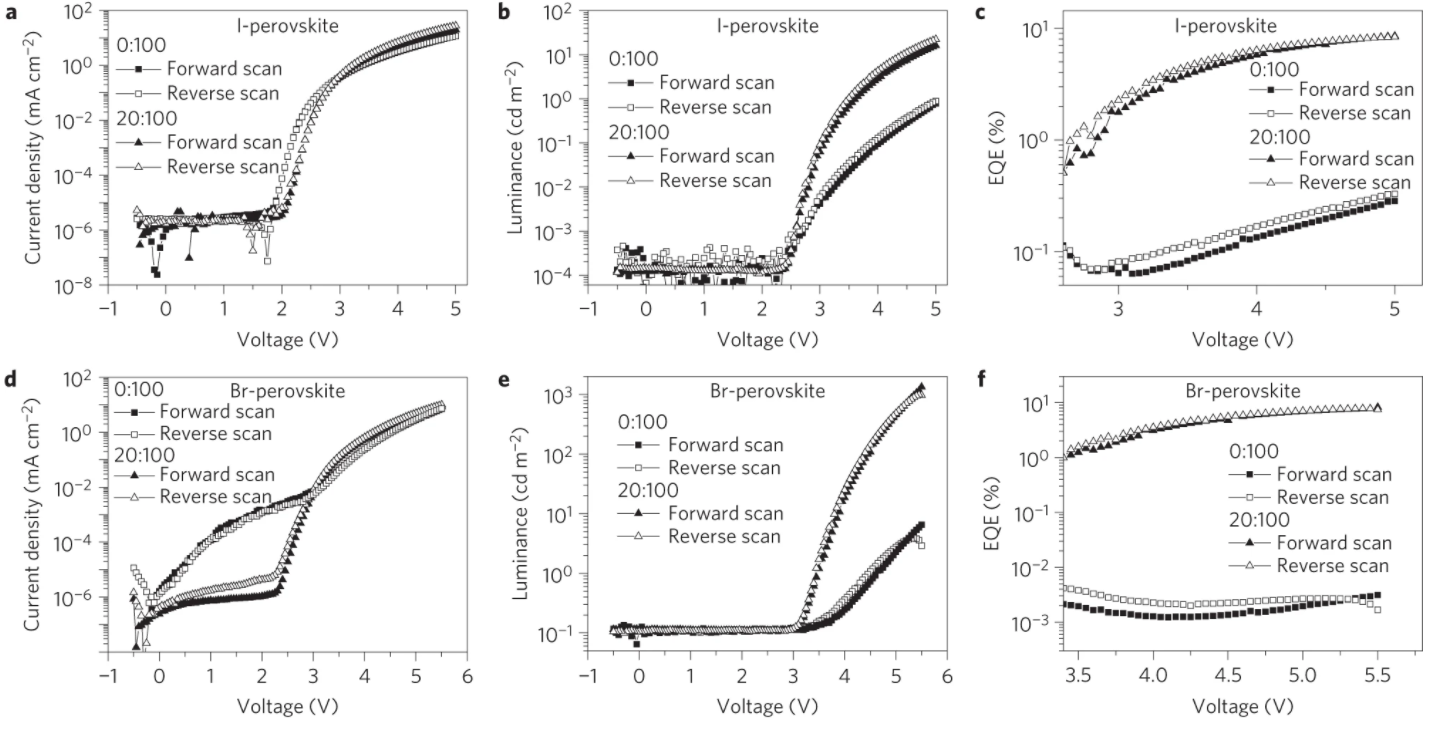
\includegraphics[width=1.0\linewidth]{pic/4.png}
		\caption{迟滞效应对$PeLED$性能的影响\cite{xiao2017efficient}
		}
	\end{figure}
\end{frame}
\subsection{$PeLED$与$OLED$和$QLED$对比}
\begin{frame}
\begin{itemize}\small{
	\item 光谱方面,$PeLED$ 和 $QLED$ 都可以通过组分调节以及量子限域效应的方法改变发光峰位,电致荧光可以从整个可见光范围延伸到近红外区域。$OLED$ 要实现发光峰位的移动则需要合成不同的发光分子,光谱范围基本集中在可见光区域。
	\item 色纯度方面,由于有机材料固有限制,$OLED(FWHW>50 nm)$ 比 $QLED$($FWHW\sim 30 nm$)和$PeLED$($FWHW< 20 nm$)都要略逊一筹,因此$PeLED $在色纯度方面表现尤其出色,能够覆盖更广的色域空间,非常适合用于高性能显示器件。
	\item 器件方面,$OLED$ 的最高效率往往在低亮度下达到,高电流高亮度情况下则伴随着显著的效率滚降,而 $QLED$ 和$PeLED$ 都报道了效率滚降很小的器件,满足了高亮度场景的使用要求。($OLED$ 与$QLED$ 目前都已经有超过百万小时寿命的器件报道,$OLED$ 更是已经投入了商业化应用,而$PeLED$的稳定性研究才刚刚起步不久,报道的最佳寿命也仅仅数百小时\cite{wang2019trifluoroacetate}。)
	\item 工艺方面,三种器件都可以通过低成本的低温溶液加工工艺生产制备,都可以兼容柔性衬底,而$OLED$ 除了溶液工艺之外还可以通过真空蒸镀的方式制备。
}
\end{itemize}
\end{frame}
\begin{frame}
	\begin{figure}[H]
		\centering
		\hspace{2em}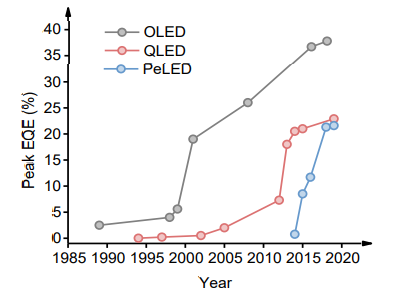
\includegraphics[width=.8\linewidth]{pic/5.png}
		\caption{$OLED, QLED, PeLED $效率发展历程
		}
	\end{figure}
\end{frame}
\subsection{钙钛矿二极管发展历程}
\begin{frame}
\begin{itemize}
	\item 1994年,日本九州大学团队第一次利用钙钛矿进行电致发光,但由于激子声子相互作用很强,只能在极低温使用。
	\item 2014 年,剑桥大学 Richard Friend 团队率先报道了室温下可工作的钙钛矿 LED。
	\item 2015 年南工大王建浦与浙大金一政团队合作研究,将 $PeLED$ 的效率提升到了 $0.8\%$(绿
	光)和 $3.5\%$(近红外)。
	\item 2017 年,普林斯顿大学 Barry Rand 等人发现通过精细调控钙钛矿前驱体溶液中加的长链铵盐的
	量,除了准二维钙钛矿之外,还可以形成自组装的钙钛矿纳米晶。
	\item 2018 年南工大王建浦团队实现了$ EQE$ 达到 $20.7\%$的近红外$PeLED$。
	\item 2018年华侨大学魏展画团队实现了 $20.3\%EQE$ 的绿光 $PeLED$。
	\item 2021年华侨大学魏展画团队实现了最高 $25.6\%EQE$ 的绿光 $PeLED$。
\end{itemize}
\end{frame}
\section{蓝光$PeLED$}
\subsection{蓝光发射钙钛矿材料}
\begin{frame}
\begin{block}{3d钙钛矿}
\begin{itemize}\small{
\item 可以通过混合不同$B$位或者$X$位元素来改变带隙大小,从而调节发光波长,但通过改变$X$位卤素元素的配比来调整带隙大小为最常用的方法。
\item 在钙钛矿结构中$X$位卤素空位为最主要的缺陷态,而$Br$与$I$元素空位形成的缺陷为浅能级缺陷,在热激发下能重新回到带边辐射复合,但$Cl$空位为高度局域化的陷阱态,有显著的非辐射复合,因此对于$Cl$空位的表面钝化非常重要。}
\end{itemize}
\end{block}
\begin{block}{钙钛矿量子点$(PeQDs)$}
\begin{itemize}
\item 钙钛矿量子点的发光性能很好,有着很高的量子产率,制备方法有热注入法、室温配体辅助再沉淀法、超声合成法等。
\item 可以通过调节卤化物组成来调节发光峰位,或者通过调节有机配体油酸的用量来调节胶体量子点的直径,从而将发光峰位调节至蓝光发射。
\end{itemize}
\end{block}
\end{frame}
\subsection{蓝光发射钙钛矿薄膜制备方法}
\begin{frame}
	\begin{figure}[H]
		\centering
		\hspace{2em}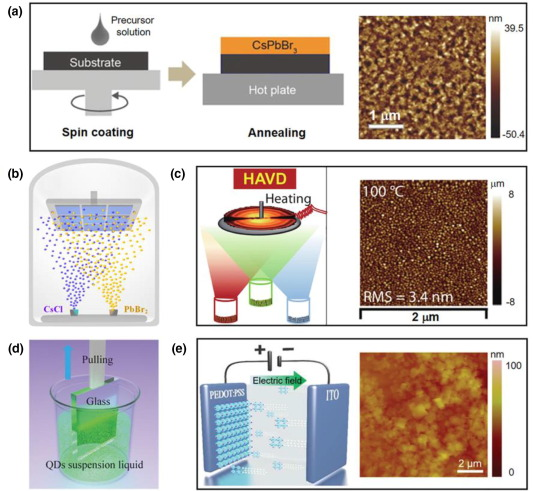
\includegraphics[width=.6\linewidth]{pic/7.jpg}
		\caption{(a)一步旋转镀膜的原理图(b)双源共蒸发示意图(c)加热辅助真空沉积示意图(d)浸涂法制备有机金属卤化物$PeQDs$薄膜示意图(e)制备$(PEA)_{2}PbBr_{4}$薄膜过程示意图\cite{zhang2021blue}
		}
	\end{figure}
\end{frame}
\subsection{如何提高蓝光$PeLED$的效率}
\begin{frame}
\begin{block}{$A$位离子掺杂}
\begin{itemize}
\item 钙钛矿材料的混合$A$位点阳离子策略可以提高钙钛矿太阳能电池的效率和稳定性,同样,钙钛矿交替的$A$位组成也可以提高$PeLED$的性能。少量的有机阳离子引入$CsPbBr_{3}$增加了钙钛矿的$PL$发射由于$Pb$抑制的金属复合中心,确认$Cs$的引入有利于蓝色$PeLED$的长期稳定。
\item $Rb$是制备蓝色钙钛矿材料最常用的$A$位阳离子掺杂剂,其半径比$Cs$小。由于钙钛矿结构的灵活性,通过改变$A$位阳离子的大小,可以对角共八面体骨架施加化学压力,从而减小了电子云之间的重叠\footnote{同样的我们可以通过增加半径大的有机阳离子减小$Pb-Cl/Br$间的电子云重叠从而改善蓝光$PL$发射},增大了钙钛矿的带隙。因此钙钛矿与$Rb$阳离子的掺杂可以调节$PL$发射向更短的波长。同时掺杂$Rb$元素可以增大$CsPbCl_{3}$的薄膜覆盖率,改善蓝色$PeLED$的光学性能。
\end{itemize}
\end{block}
\end{frame}
\begin{frame}
	\begin{figure}[H]
		\centering
		\hspace{2em}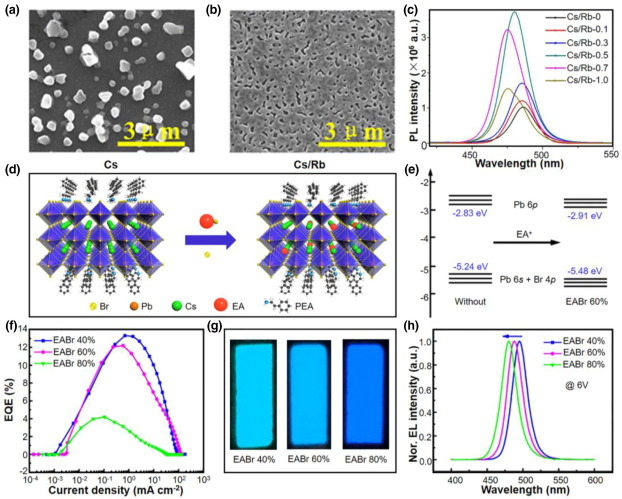
\includegraphics[width=.7\linewidth]{pic/8.jpg}
		\caption{(a)(b)掺杂与不掺杂薄膜的形态(c)掺杂$Rb$不同浓度的$PL$谱(d)(e)掺杂$Rb$后的晶体结构与能带结构,(f)(g)(h)$A$位离子掺杂$EA$后光谱表征\cite{zhang2021blue}
		}
	\end{figure}
\end{frame}
\begin{frame}
\begin{block}{$B$位离子掺杂}
\begin{itemize}\small{
\item 由于位于共角八面体中心的$B$位元素不仅通过改变八面体旋转或倾斜的程度影响钙钛矿的晶相,而且还决定了它们的电子能带结构,不同金属离子部分取代$Pb^{2+}$离子是调节钙钛矿材料发射波长,提高其稳定性和光电性能的一种可能方法。
\item 通过在钙钛矿量子点中掺杂少量$Mn$掺杂剂,将$Mn$掺杂$CsPbBr_{3}$薄膜的$PLQY$提高了3倍以上,同时保持了良好的纯蓝色发射。
\item 通过将$YCl_{3}$加入2d钙钛矿中,该$PeLED$在485nm处显示出稳定的发射峰,记录的$EQE$高达11.0\%。添加的$YCl_{3}$不仅掺杂到钙钛矿晶格中,而且还存在于晶界和晶面,有效地限制了载流子,有利于辐射重组。
\item $Ni$掺杂可以有效消除卤化物空位等固有缺陷(增加缺陷形成能\footnote{$Cu^{2+}$也能有相同的效果}),并导致晶格的近程序增加,没有在带隙中引入深阱态,可以造成局部结构有序改善和$PLQY$显著增强。}
\end{itemize}
\end{block}
\end{frame}
\begin{frame}
	\begin{figure}[H]
		\centering
		\hspace{2em}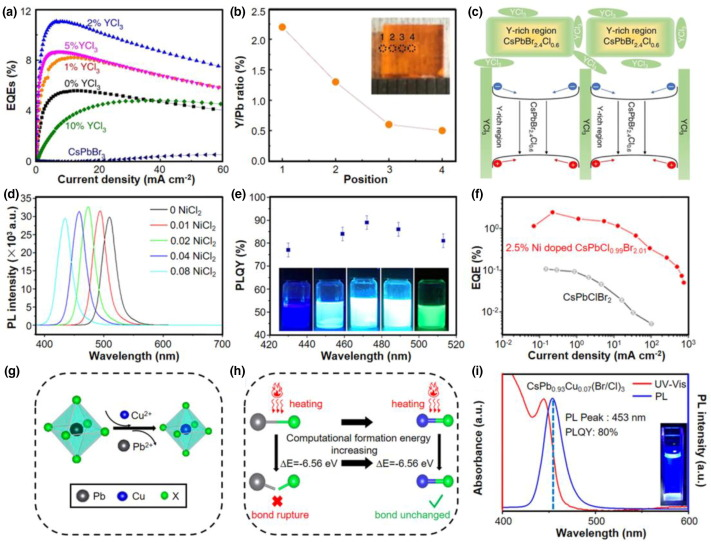
\includegraphics[width=.65\linewidth]{pic/9.jpg}
		\caption{(a)不同$YCl_{3}$配比下$PeLED$的$EQE$曲线(b) $CsPbBr_{3}$钙钛矿晶体不同位置的$Y/Pb$比值(c)薄膜中Y离子的梯度分布及其对颗粒中载流子的限制作用示意图。(d)(e)(f)不同掺杂$Ni$离子下参数的表征(g)(h)(i)掺杂$Cu$离子下的光谱参数表征
        \cite{zhang2021blue}
		}
	\end{figure}
\end{frame}
\begin{frame}
\begin{block}{蓝光$PeLED$的表面配体I}
\begin{itemize}
\item 在胶体钙钛矿量子点的合成中,表面配体可以保持颗粒在溶液中的单分散性,钝化钙钛矿量子点的表面缺陷,提高材料的稳定性,$OA$和$OAm$是合成钙钛矿量子点常用的两种表面配体。
\item $OA$可以抑制钙钛矿纳米碳化物的团聚,提高其稳定性;$OAm$可以通过影响晶化动力学来防止钙钛矿聚合形成大晶粒。但是这些配体表现出高度动态和松散的结合,在隔离和纯化过程中很容易从表面脱落,导致量子点的降解。
\end{itemize}
\end{block}
\end{frame}
\begin{frame}
\begin{block}{蓝光$PeLED$的表面配体II}
\begin{itemize}
\item 另一种增强载体注入和转运以及改善胶体钙钛矿发光特性的有效方法是通过引入高迁移率的无机配体来部分替代有机配体,从而提高薄膜的电导率和辐射重组。通过引入碱金属$K^{+}$作为一种新型配体,并通过减少绝缘有机配体可以得到了具有优越电导率的钙钛矿薄膜。同时发现利用$PrCl_{3}$对$PeLED$进行了预优化,不仅可以有效地钝化表面的$Cl$空位,还可以通过取代它们来适当地减少它们表面的长链有机配体。
\item 还可以采用了一种三辛基氧化膦$(TOPO)$介导的方法,通过改变$TOPO$的数量,可以有效地调节表面配体的浓度。$TOPO$可以很容易地与游离$OA$中的酸性质子结合,形成脱质子油酸基的酸碱络合物,而脱质子油酸基可以很容易地去除,此外,$TOPO-PbBr_{2}$的形成可以减少欠配位$Pb^{2+}$。
\end{itemize}
\end{block}
\end{frame}
\subsection{蓝光$PeLED$的挑战与困难}
\begin{frame}
\begin{block}{真正的蓝光$PeLED$}
	\begin{figure}[H]
		\centering
		\hspace{2em}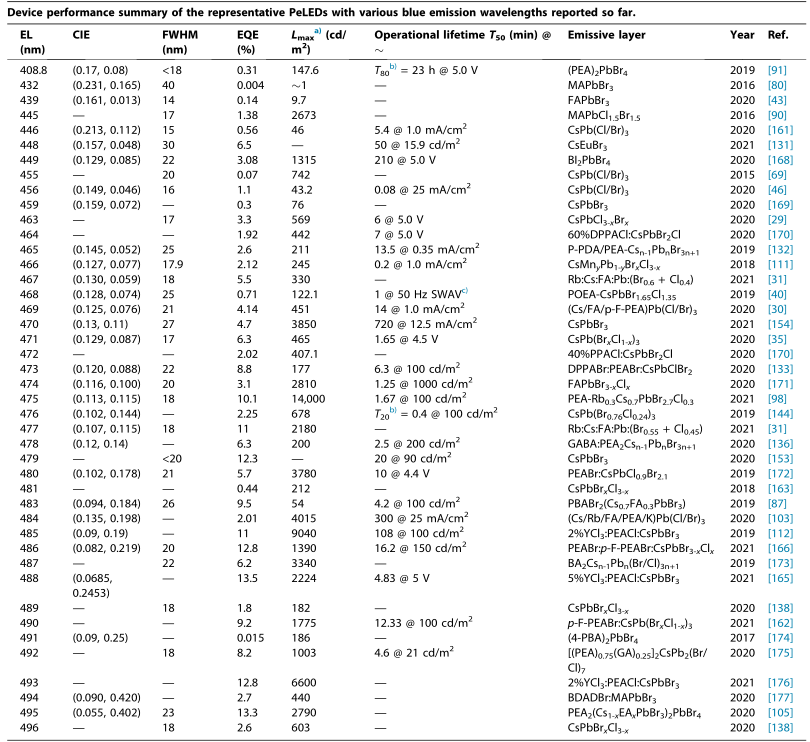
\includegraphics[width=.56\linewidth]{pic/10.png}
	\end{figure}
\begin{itemize}
\item \tiny{为了使$PeLED$的发射波长调整到真正蓝光范围($455-470nm$),要么需要过量的$Cl^{-}$取代$Br^{-}$,要么需要减小钙钛矿量子点的尺寸以获得更高的激子束缚能。然而含$Cl$元素合成的混合卤素钙钛矿膜含有大量的缺陷,长链配体的存在减小了钙钛矿量子点的尺寸,但是阻碍了电荷载体的注入和输运。}
\end{itemize}
\end{block}
\end{frame}
\begin{frame}
\begin{block}{光谱稳定性问题}
\begin{itemize}
\item 钙钛矿材料离子迁移是一个值得关注的问题,会导致混合卤化物$PeLED$的光谱不稳定,由于卤化物的分离,光谱稳定性是实现稳定的蓝光发射$PeLED$的重要挑战之一。
\item 制备混合阳离子钙钛矿是稳定混合卤化物发射光谱的有效方法。例如,已有研究表明,由于晶格形成能的增加,可以通过一种具有较小离子半径的替代二价金属元素来减少其中卤素空位缺陷的形成,从而使得离子迁移效应的影响减小。
\item 为实现具有高效蓝光发射和良好光谱稳定性的$PeLED$,在钙钛矿前驱体溶液中引入不同的配体,影响其结晶过程,从而调节蓝色发射波长,并通过操纵堆积的体积大的有机配体之间的范德瓦尔斯相互作用来提高光谱稳定性。
\end{itemize}
\end{block}
\end{frame}
\begin{frame}
\begin{block}{$Pb$元素的毒性问题}
\begin{itemize}
\item $Pb$元素的毒性是$PeLED$商业化应用面临的另一个挑战。含铅体系相对稳定,降解时间较长,会对环境和机体造成不可弥补的破坏。因此,有必要用其他低毒性或无毒的金属元素替代铅。目前发现$Sn^{2+}$与$Pb^{2+}$在半径等许多方面具有相似之处,是$Pb^{2+}$的理想替代品,但$Sn^{2+}$在空气中容易被氧化为$Sn^{4+}$,从而产生不良的高自由载流子密度,导致钙钛矿膜$PL$猝灭,其余元素作为$Pb$元素的替代元素制作的器件$EQE$及稳定性均远低于含$Pb$器件。
\item 另一种类型的是卤化物双钙钛矿,然而卤化物双钙钛矿是间接带隙半导体,具有宽$PL$,不能用作电致发光器件的发射器,也不适合用于超高清显示应用。
\end{itemize}
\end{block}
\end{frame}
\section{总结}
\subsection{钙钛矿材料的优势}
\begin{frame}
\begin{itemize}
	\item 发光可以在$400-800 nm$ 的范围内连续可调,覆盖了整个可见光区域。
	\item 直接带隙半导体导致荧光谱宽很窄,发光色纯度高。
	\item 钙钛矿材料大部分为宽禁带半导体材料,除了光学性质外还有很好的热导率,击穿场强及电子饱和迁移速率。
	\item 钙钛矿材料的荧光量子产率较高,且在较小的激发密度下的荧光量子产率不会有较大的减小。
	\item 钙钛矿材料的单线态与三线态能级差别很小,能实现快速转换,因此允许光学跃迁态(单线态)比例很高。
	\item 高电流密度及低电流密度下的$PeLED$的发光效率较高,没有太大差别。
\end{itemize}
\end{frame}

\subsection{钙钛矿材料的缺点}
\begin{frame}
\begin{itemize}
	\item $PeLED$的离子迁移问题:当有外加电场存在时,钙钛矿中的离子(主要是卤素离子)会从晶界、表面等存在大量缺陷的地方开始发生移动,从而导致器件性能的衰减。
	\item $PeLED$的迟滞现象:受到离子迁移的影响,$PeLED$在电压正扫和反扫是不重合的,导致性能不稳定。
	\item 由于钙钛矿材料的消光系数很高及器件表面有强烈的表面等离子激元共振吸收,导致钙钛矿器件的出光效率很低。
	\item 目前$PeLED$中蓝光$LED$方面器件的光谱稳定性欠佳(离子迁移现象引起),且器件寿命有待提高,离商用化还有较大的距离。
	\item 成膜后的钙钛矿纳米结构为热力学不稳定结构,需要大量配体平衡,但也阻碍空穴电子层的载流子运输。
	\item 目前钙钛矿材料只有在$Pb^{2+}$存在时的性能较好,但$Pb^{2+}$严重污染环境。
\end{itemize}
\end{frame}	
    \section{参考文献}	
    \begin{frame}[allowframebreaks]{参考文献}
    \printbibliography[heading=none]
    \end{frame}
	\begin{frame}
		\begin{center}
			{\Huge\calligra Questions?}
		\end{center}
	\end{frame}
	\begin{frame}
		\begin{center}
			{\Huge\calligra Thanks!}
		\end{center}
	\end{frame}
\end{document}
